% answers.tex —— 2007 年·普通高等学校招生考试·浙江卷·文科 · 参考答案与详细解析片段
% 由 tools/generate_projects.py 依来源总账自 2007/2007_数学真题_浙江文_试题.md + 2007/2007_数学真题_浙江文_解析正文.md + 2007/2007_数学真题_浙江文_答案要点.md 生成，勿手改（改源 MD 后重跑）


\begin{gktip}
固定候选 PDF 仅含题面，无答案、解析和评分标准，原卷亦未标注分值；以下为非官方编者独立推导，官方答案字段为空。来源发布者、出版者、版次与官方身份均未核。
\end{gktip}

\begin{answer}
\gksolhead{1}{}

\textbf{题目}：

设全集 $U=\{1,3,5,6,8\}$，$A=\{1,6\}$，$B=\{5,6,8\}$，则 $(\complement_UA)\cap B=$（　）

（A）$\{6\}$

（B）$\{5,8\}$

（C）$\{6,8\}$

（D）$\{3,5,6,8\}$

\Needspace{4\baselineskip}
\textbf{解析}

\Needspace{5\baselineskip}
$\complement_UA=\{3,5,8\}$，与 $B=\{5,6,8\}$ 取交集：

\nopagebreak[4]
\[(\complement_UA)\cap B=\{5,8\}.\]

\gkanswer{答案：B。}

\end{answer}
\begin{answer}
\gksolhead{2}{}

\textbf{题目}：

已知 $\cos\left(\dfrac{\pi}{2}+\varphi\right)=\dfrac{\sqrt3}{2}$，且 $|\varphi|<\dfrac{\pi}{2}$，则 $\tan\varphi=$（　）

（A）$-\dfrac{\sqrt3}{3}$

（B）$\dfrac{\sqrt3}{3}$

（C）$-\sqrt3$

（D）$\sqrt3$

\Needspace{4\baselineskip}
\textbf{解析}

\nopagebreak[4]
\[\cos\left(\frac{\pi}{2}+\varphi\right)=-\sin\varphi=\frac{\sqrt3}{2},\]

\Needspace{5\baselineskip}
故

\nopagebreak[4]
\[\sin\varphi=-\frac{\sqrt3}{2}.\]

\Needspace{5\baselineskip}
由 $|\varphi|<\dfrac{\pi}{2}$ 得 $\varphi=-\dfrac{\pi}{3}$，故

\nopagebreak[4]
\[\tan\varphi=-\sqrt3.\]

\gkanswer{答案：C。}

\end{answer}
\begin{answer}
\gksolhead{3}{}

\textbf{题目}：

“$x>1$”是“$x^2>x$”的（　）

（A）充分而不必要条件

（B）必要而不充分条件

（C）充分必要条件

（D）既不充分也不必要条件

\Needspace{4\baselineskip}
\textbf{解析}

\nopagebreak[4]
\[x^2>x\ \Leftrightarrow\ x(x-1)>0\ \Leftrightarrow\ x>1\ \text{\text{或}}\ x<0.\]

$x>1$ 能推出 $x^2>x$，但 $x^2>x$ 不一定有 $x>1$（如 $x=-1$），故为充分而不必要条件。

\gkanswer{答案：A。}

\end{answer}
\begin{answer}
\gksolhead{4}{}

\textbf{题目}：

直线 $x-2y+1=0$ 关于直线 $x=1$ 对称的直线方程是（　）

（A）$x+2y-1=0$

（B）$2x+y-1=0$

（C）$2x+y-3=0$

（D）$x+2y-3=0$

\Needspace{4\baselineskip}
\textbf{解析}

\Needspace{5\baselineskip}
关于 $x=1$ 对称，把 $x$ 换成 $2-x$：

\nopagebreak[4]
\[(2-x)-2y+1=0\ \Rightarrow\ -x-2y+3=0,\]

\Needspace{5\baselineskip}
即

\nopagebreak[4]
\[x+2y-3=0.\]

\gkanswer{答案：D。}

\end{answer}
\begin{answer}
\gksolhead{5}{}

\textbf{题目}：

要在边长为 $16$ 米的正方形草坪上安装喷水龙头，使整个草坪都能喷洒到水。假设每个喷水龙头的喷洒范围都是半径为 $6$ 米的圆面，则需安装这种喷水龙头的个数最少是（　）
\nopagebreak[4]
\begin{center}% 2007 年浙江卷文科第 5 题：边长 16 米的正方形草坪与喷水龙头示意。
% 来源 PDF：gaokaomath-src/普通高考/2007/2007浙江文.pdf
% SHA-256：31c1d0d79ba11a3644a27b5ee3781f52caaf831209e8da63ddd8d7019cd06995
% 原页：2007浙江文.pdf 第 1 页（A3 三栏）第 1 栏，书页码 419。
% 重绘依据：按原页正方形草坪与中心喷水圆面的透视重绘。
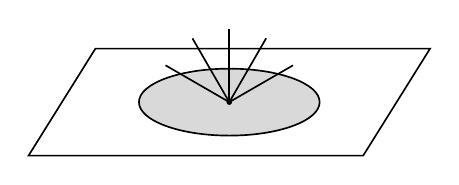
\begin{tikzpicture}[scale=0.85, semithick,
  every node/.style={inner sep=1pt}]

  % 正方形草坪（斜投影）
  \draw (0,0) -- (5,0) -- (6,1.6) -- (1,1.6) -- cycle;

  % 喷水圆面
  \fill[gray!30] (3,0.8) ellipse (1.35 and 0.5);
  \draw (3,0.8) ellipse (1.35 and 0.5);
  \fill (3,0.8) circle (1.2pt);

  % 水花射线
  \foreach \a in {30,60,90,120,150} {
    \draw (3,0.8) -- ++(\a:1.1);
  }
\end{tikzpicture}
\end{center}
\nopagebreak[4]
（A）$6$

（B）$5$

（C）$4$

（D）$3$

\Needspace{4\baselineskip}
\textbf{解析}

一个半径 $6$ 的圆无法同时覆盖正方形两个相距 $16$ 的顶点（直径 $12<16$），故四个顶点需由不同圆覆盖；三个圆至多覆盖三个顶点，故至少 $4$ 个。

\Needspace{5\baselineskip}
取四个圆心在四个边长为 $8$ 的小正方形中心，每个小正方形的顶点到中心距离

\nopagebreak[4]
\[\sqrt{4^2+4^2}=4\sqrt2<6,\]

故 $4$ 个圆可覆盖整个草坪。最少为 $4$ 个。

\gkanswer{答案：C。}

\end{answer}
\begin{answer}
\gksolhead{6}{}

\textbf{题目}：

$\left(\sqrt x-\dfrac1x\right)^9$ 展开式中的常数项是（　）

（A）$-36$

（B）$36$

（C）$-84$

（D）$84$

\Needspace{4\baselineskip}
\textbf{解析}

\Needspace{5\baselineskip}
通项

\nopagebreak[4]
\[\mathrm C_9^k(\sqrt x)^{9-k}\left(-\frac1x\right)^k
=\mathrm C_9^k(-1)^k x^{\frac{9-k}{2}-k}
=\mathrm C_9^k(-1)^k x^{\frac{9-3k}{2}}.\]

\Needspace{5\baselineskip}
令 $\dfrac{9-3k}{2}=0$，得 $k=3$。常数项为

\nopagebreak[4]
\[\mathrm C_9^3(-1)^3=-84.\]

\gkanswer{答案：C。}

\end{answer}
\begin{answer}
\gksolhead{7}{}

\textbf{题目}：

若 $P$ 是两条异面直线 $l$，$m$ 外的任意一点，则（　）

（A）过点 $P$ 有且仅有一条直线与 $l$，$m$ 都平行

（B）过点 $P$ 有且仅有一条直线与 $l$，$m$ 都垂直

（C）过点 $P$ 有且仅有一条直线与 $l$，$m$ 都相交

（D）过点 $P$ 有且仅有一条直线与 $l$，$m$ 都异面

\Needspace{4\baselineskip}
\textbf{解析}

异面直线 $l$，$m$ 的方向向量不平行，过 $P$ 且与两者都垂直的直线方向唯一（两方向向量的叉乘方向），故有且仅有一条；其余选项均不恒成立。

\gkanswer{答案：B。}

\end{answer}
\begin{answer}
\gksolhead{8}{}

\textbf{题目}：

甲，乙两人进行乒乓球比赛，比赛规则为“$3$ 局 $2$ 胜”，即以先赢 $2$ 局者为胜。根据经验，每局比赛中甲获胜的概率为 $0.6$，则本次比赛甲获胜的概率是（　）

（A）$0.216$

（B）$0.36$

（C）$0.432$

（D）$0.648$

\Needspace{4\baselineskip}
\textbf{解析}

甲获胜的情况：

\begin{itemize}
\item 连胜两局：$0.6^2=0.36$；
\item 前两局一胜一负、第三局胜：$2\times0.6\times0.4\times0.6=0.288$。
\end{itemize}

\Needspace{5\baselineskip}
合计

\nopagebreak[4]
\[0.36+0.288=0.648.\]

\gkanswer{答案：D。}

\end{answer}
\begin{answer}
\gksolhead{9}{}

\textbf{题目}：

若非零向量 $\boldsymbol a$，$\boldsymbol b$ 满足 $|\boldsymbol a-\boldsymbol b|=|\boldsymbol b|$，则（　）

（A）$|2\boldsymbol b|<|\boldsymbol a-2\boldsymbol b|$

（B）$|2\boldsymbol b|<|\boldsymbol a-2\boldsymbol b|$

（C）$|2\boldsymbol a|>|2\boldsymbol a-\boldsymbol b|$

（D）$|2\boldsymbol a|<|2\boldsymbol a-\boldsymbol b|$

\Needspace{4\baselineskip}
\textbf{解析}

\Needspace{5\baselineskip}
由 $|\boldsymbol a-\boldsymbol b|=|\boldsymbol b|$ 平方得

\nopagebreak[4]
\[\boldsymbol a^2-2\boldsymbol a\cdot\boldsymbol b=0\ \Rightarrow\ \boldsymbol a\cdot\boldsymbol b=\frac{\boldsymbol a^2}{2}.\]

\Needspace{5\baselineskip}
于是

\nopagebreak[4]
\[|\boldsymbol a-2\boldsymbol b|^2=\boldsymbol a^2-4\boldsymbol a\cdot\boldsymbol b+4\boldsymbol b^2=4\boldsymbol b^2-\boldsymbol a^2<4\boldsymbol b^2=|2\boldsymbol b|^2,\]

即 $|2\boldsymbol b|>|\boldsymbol a-2\boldsymbol b|$。

【源疑点：原页（A）（B）均印作 $|2\boldsymbol b|<|\boldsymbol a-2\boldsymbol b|$，按题设应有 $|2\boldsymbol b|>|\boldsymbol a-2\boldsymbol b|$；此处按命题意图取 B（B 应为 $>$）。】

\gkanswer{答案：B。}

\end{answer}
\begin{answer}
\gksolhead{10}{}

\textbf{题目}：

已知双曲线 $\dfrac{x^2}{a^2}-\dfrac{y^2}{b^2}=1$（$a>0$，$b>0$）的左、右焦点分别为 $F_1$，$F_2$，$P$ 是准线上一点，且 $PF_1\perp PF_2$，$|PF_1|\cdot|PF_2|=4ab$，则双曲线的离心率是（　）

（A）$\sqrt2$

（B）$\sqrt3$

（C）$2$

（D）$3$

\Needspace{4\baselineskip}
\textbf{解析}

\Needspace{5\baselineskip}
设 $P$ 在右准线 $x=\dfrac{a^2}{c}$ 上。由 $PF_1\perp PF_2$，$P$ 在以 $F_1F_2$ 为直径的圆上：

\nopagebreak[4]
\[x_P^2+y_P^2=c^2.\]

\Needspace{5\baselineskip}
代入 $x_P=\dfrac{a^2}{c}$ 得

\nopagebreak[4]
\[y_P^2=c^2-\frac{a^4}{c^2}.\]

\Needspace{5\baselineskip}
于是

\nopagebreak[4]
\[|PF_1|^2=\left(\frac{a^2}{c}+c\right)^2+y_P^2=2(a^2+c^2),\]

\nopagebreak[4]
\[|PF_2|^2=\left(\frac{a^2}{c}-c\right)^2+y_P^2=2(c^2-a^2).\]

\Needspace{5\baselineskip}
由 $|PF_1||PF_2|=4ab$：

\nopagebreak[4]
\[2\sqrt{c^4-a^4}=4ab\ \Rightarrow\ c^4-a^4=4a^2b^2=4a^2(c^2-a^2).\]

\Needspace{5\baselineskip}
令 $e=\dfrac ca$，两边除以 $a^4$：

\nopagebreak[4]
\[e^4-1=4(e^2-1)\ \Rightarrow\ (e^2-1)(e^2-3)=0.\]

$e>1$，故 $e=\sqrt3$。

\gkanswer{答案：B。}

\end{answer}
\begin{answer}
\gksolhead{11}{}

\textbf{题目}：

函数 $y=\dfrac{x^2}{x^2+1}$（$x\in\mathbf R$）的值域是\gkblank{}。

\Needspace{4\baselineskip}
\textbf{解析}

\nopagebreak[4]
\[y=\frac{x^2}{x^2+1}=1-\frac1{x^2+1}.\]

\Needspace{5\baselineskip}
$x^2+1\geqslant1$，故 $0<\dfrac1{x^2+1}\leqslant1$，从而

\nopagebreak[4]
\[0\leqslant y<1.\]

\gkanswer{答案：$[0,1)$。}

\end{answer}
\begin{answer}
\gksolhead{12}{}

\textbf{题目}：

若 $\sin\theta+\cos\theta=\dfrac15$，则 $\sin2\theta$ 的值是\gkblank{}。

\Needspace{4\baselineskip}
\textbf{解析}

\Needspace{5\baselineskip}
两边平方：

\nopagebreak[4]
\[1+\sin2\theta=\frac1{25},\]

\Needspace{5\baselineskip}
故

\nopagebreak[4]
\[\sin2\theta=-\frac{24}{25}.\]

\gkanswer{答案：$-\dfrac{24}{25}$。}

\end{answer}
\begin{answer}
\gksolhead{13}{}

\textbf{题目}：

某校有学生 $2000$ 人，其中高三学生 $500$ 人。为了解学生的身体素质情况，采用按年级分层抽样的方法，从该校学生中抽取一个 $200$ 人的样本。则样本中高三学生的人数为\gkblank{}。

\Needspace{4\baselineskip}
\textbf{解析}

\Needspace{5\baselineskip}
抽样比为 $\dfrac{200}{2000}=\dfrac1{10}$，高三学生人数为

\nopagebreak[4]
\[500\times\frac1{10}=50.\]

\gkanswer{答案：$50$。}

\end{answer}
\begin{answer}
\gksolhead{14}{}

\textbf{题目}：

$z=2x+y$ 中的 $x$，$y$ 满足约束条件 $\begin{cases}x-2y+5\geqslant0,\\ 3-x\geqslant0,\\ x+y\geqslant0,\end{cases}$ 则 $z$ 的最小值是\gkblank{}。

\Needspace{4\baselineskip}
\textbf{解析}

可行域由三条直线围成。顶点：

\begin{itemize}
\item $x=3$ 与 $x+y=0$：$(3,-3)$，$z=3$；
\item $x=3$ 与 $x-2y+5=0$：$(3,4)$，$z=10$；
\item $x+y=0$ 与 $x-2y+5=0$：$\left(-\dfrac53,\dfrac53\right)$，$z=-\dfrac53$。
\end{itemize}

故最小值为 $-\dfrac53$。

\gkanswer{答案：$-\dfrac53$。}

\end{answer}
\begin{answer}
\gksolhead{15}{}

\textbf{题目}：

曲线 $y=x^3-2x^2-4x+2$ 在点 $(1,-3)$ 处的切线方程是\gkblank{}。

\Needspace{4\baselineskip}
\textbf{解析}

\nopagebreak[4]
\[y'=3x^2-4x-4,\qquad y'(1)=3-4-4=-5.\]

\Needspace{5\baselineskip}
切线：

\nopagebreak[4]
\[y+3=-5(x-1)\ \Rightarrow\ y=-5x+2.\]

\gkanswer{答案：$y=-5x+2$。}

\end{answer}
\begin{answer}
\gksolhead{16}{}

\textbf{题目}：

某书店有 $11$ 种杂志，$2$ 元 $1$ 本的 $8$ 种，$1$ 元 $1$ 本的 $3$ 种。小张用 $10$ 元钱买杂志（每种至多买一本，$10$ 元钱刚好用完），则不同买法的种数是\gkblank{}。（用数字作答）

\Needspace{4\baselineskip}
\textbf{解析}

\Needspace{5\baselineskip}
设买 $2$ 元杂志 $k$ 本、$1$ 元杂志 $m$ 本：

\nopagebreak[4]
\[2k+m=10,\qquad 0\leqslant k\leqslant8,\ 0\leqslant m\leqslant3.\]

\Needspace{5\baselineskip}
$m=10-2k\in[0,3]$ 给出 $k=4$（$m=2$）或 $k=5$（$m=0$）。买法数为

\nopagebreak[4]
\[\mathrm C_8^4\mathrm C_3^2+\mathrm C_8^5=70\times3+56=266.\]

\gkanswer{答案：$266$。}

\end{answer}
\begin{answer}
\gksolhead{17}{}

\textbf{题目}：

已知点 $O$ 在二面角 $\alpha-AB-\beta$ 的棱上，点 $P$ 在 $\alpha$ 内，且 $\angle POB=45^\circ$。若对于 $\beta$ 内异于 $O$ 的任意一点 $Q$，都有 $\angle POQ\geqslant45^\circ$，则二面角 $\alpha-AB-\beta$ 的大小是\gkblank{}。

\Needspace{4\baselineskip}
\textbf{解析}

设二面角为 $\varphi$。在 $\alpha$ 内取 $OB\perp AB$，$OP$ 与 $OB$ 成 $45^\circ$。$\beta$ 内离 $OP$ 最近的射线与 $OP$ 的夹角为 $OP$ 与平面 $\beta$ 的夹角；题设要求该最小角为 $45^\circ$。

$OP$ 与 $\beta$ 的夹角为 $45^\circ$ 当且仅当 $OP$ 与 $\beta$ 内垂直于棱的射线 $OB'$ 的夹角为 $45^\circ$，即 $\varphi=45^\circ$。

\gkanswer{答案：$45^\circ$。}

\end{answer}
\begin{answer}
\gksolhead{18}{}

\textbf{题目}：

已知 $\triangle ABC$ 的周长为 $\sqrt2+1$，且 $\sin A+\sin B=\sqrt2\sin C$。

（1）求边 $AB$ 的长；

（2）若 $\triangle ABC$ 的面积为 $\dfrac16\sin C$，求角 $C$ 的度数。

\Needspace{4\baselineskip}
\textbf{解析}

\Needspace{5\baselineskip}
（1）由正弦定理，$\sin A+\sin B=\sqrt2\sin C$ 化为

\nopagebreak[4]
\[a+b=\sqrt2c.\]

\Needspace{5\baselineskip}
周长

\nopagebreak[4]
\[a+b+c=(\sqrt2+1)c=\sqrt2+1,\]

故 $c=AB=1$。

\Needspace{5\baselineskip}
（2）面积

\nopagebreak[4]
\[S=\frac12ab\sin C=\frac16\sin C\ \Rightarrow\ ab=\frac13.\]

\Needspace{5\baselineskip}
又 $a+b=\sqrt2$，由余弦定理：

\nopagebreak[4]
\[c^2=a^2+b^2-2ab\cos C=(a+b)^2-2ab(1+\cos C).\]

\Needspace{5\baselineskip}
代入 $c=1$，$ab=\dfrac13$：

\nopagebreak[4]
\[1=2-\frac23(1+\cos C)\ \Rightarrow\ \cos C=\frac12,\]

故 $C=60^\circ$。

\gkanswer{答案：（1）$AB=1$；（2）$C=60^\circ$。}

\end{answer}
\begin{answer}
\gksolhead{19}{}

\textbf{题目}：

已知数列 $\{a_n\}$ 中的相邻两项 $a_{2k-1}$，$a_{2k}$ 是关于 $x$ 的方程 $x^2-(3k+2^k)x+3k\cdot2^k=0$ 的两个根，且 $a_{2k-1}\leqslant a_{2k}$（$k=1,2,3,\cdots$）。

（1）求 $a_1$，$a_3$，$a_5$，$a_7$ 及 $a_{2n}$（$n\geqslant4$）（不必证明）；

（2）求数列 $\{a_n\}$ 的前 $2n$ 项和 $S_{2n}$。

\Needspace{4\baselineskip}
\textbf{解析}

（1）方程两根为 $3k$ 与 $2^k$，按 $a_{2k-1}\leqslant a_{2k}$ 排序：

\begin{itemize}
\item $k=1$：$\{2,3\}$，$a_1=2$，$a_2=3$；
\item $k=2$：$\{4,6\}$，$a_3=4$，$a_4=6$；
\item $k=3$：$\{8,9\}$，$a_5=8$，$a_6=9$；
\item $k=4$：$\{12,16\}$，$a_7=12$，$a_8=16$。
\end{itemize}

$n\geqslant4$ 时 $2^n>3n$，故 $a_{2n-1}=3n$，$a_{2n}=2^n$。

\Needspace{5\baselineskip}
（2）每一对的和

\nopagebreak[4]
\[a_{2k-1}+a_{2k}=3k+2^k.\]

\Needspace{5\baselineskip}
故

\nopagebreak[4]
\[S_{2n}=\sum_{k=1}^n(3k+2^k)=3\cdot\frac{n(n+1)}2+(2^{n+1}-2).\]

\gkanswer{答案：（1）$a_1=2$，$a_3=4$，$a_5=8$，$a_7=12$，$a_{2n}=2^n$（$n\geqslant4$）；（2）$S_{2n}=\dfrac{3n(n+1)}2+2^{n+1}-2$。}

\end{answer}
\begin{answer}
\gksolhead{20}{}

\textbf{题目}：

在如图所示的几何体中，$EA\perp$ 平面 $ABC$，$DB\perp$ 平面 $ABC$，$AC\perp BC$，且 $AC=BC=BD=2AE$，$M$ 是 $AB$ 的中点。

（1）求证：$CM\perp EM$；

（2）求 $DE$ 与平面 $EMC$ 所成角的正切值。
\nopagebreak[4]
\begin{center}% 2007 年浙江卷文科第 20 题：EA、DB 均垂直于平面 ABC，AC⊥BC，M 为 AB 中点。
%   按 AC=BC=2、AE=1、BD=2 的示意比例绘制。
% 来源 PDF：gaokaomath-src/普通高考/2007/2007浙江文.pdf
% SHA-256：31c1d0d79ba11a3644a27b5ee3781f52caaf831209e8da63ddd8d7019cd06995
% 原页：2007浙江文.pdf 第 2 页（A3 三栏）第 1 栏，书页码 420。
% 重绘依据：按原页 C、A、B 底面与 E、D 的竖直位置重绘。
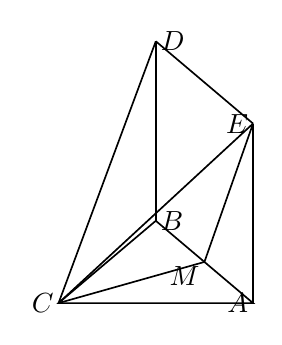
\begin{tikzpicture}[scale=0.95, semithick,
  every node/.style={inner sep=1.5pt}]

  \coordinate (C) at (0,0);
  \coordinate (A) at (2.6,0);
  \coordinate (B) at (1.3,1.1);
  \coordinate (E) at (2.6,2.4);
  \coordinate (D) at (1.3,3.5);
  \coordinate (M) at (1.95,0.55);

  % 底面
  \draw (C) -- (A) -- (B) -- cycle;
  % 竖直线
  \draw (A) -- (E);
  \draw (B) -- (D);
  % 上方连线
  \draw (E) -- (D);
  \draw (E) -- (C);
  \draw (D) -- (C);
  % 中点 M 相关
  \draw (C) -- (M);
  \draw (E) -- (M);

  \node[left] at (C) {$C$};
  \node[left] at (A) {$A$};
  \node[right] at (B) {$B$};
  \node[left] at (E) {$E$};
  \node[right] at (D) {$D$};
  \node[below left] at (M) {$M$};
\end{tikzpicture}
\end{center}
\nopagebreak[4]
\Needspace{4\baselineskip}
\textbf{解析}

\Needspace{5\baselineskip}
设 $AC=BC=2$，则 $AE=1$，$BD=2$。取 $C$ 为原点，$CA$，$CB$ 为 $x$，$y$ 轴，垂直底面向上的方向为 $z$ 轴：

\nopagebreak[4]
\[C(0,0,0),\ A(2,0,0),\ B(0,2,0),\]

\nopagebreak[4]
\[E(2,0,1),\ D(0,2,2),\ M(1,1,0).\]

\Needspace{5\baselineskip}
（1）

\nopagebreak[4]
\[\overrightarrow{CM}=(1,1,0),\qquad \overrightarrow{EM}=(1,-1,1),\]

\nopagebreak[4]
\[\overrightarrow{CM}\cdot\overrightarrow{EM}=1-1+0=0,\]

故 $CM\perp EM$。

\Needspace{5\baselineskip}
（2）平面 $EMC$ 内

\nopagebreak[4]
\[\overrightarrow{MC}=(-1,-1,0),\qquad \overrightarrow{ME}=(1,-1,1).\]

\Needspace{5\baselineskip}
法向量

\nopagebreak[4]
\[\boldsymbol n=\overrightarrow{MC}\times\overrightarrow{ME}=(-1,1,2).\]

\nopagebreak[4]
\[\overrightarrow{DE}=(2,-2,-1).\]

\Needspace{5\baselineskip}
设 $DE$ 与平面所成角为 $\varphi$，则

\nopagebreak[4]
\[\sin\varphi=\frac{|\overrightarrow{DE}\cdot\boldsymbol n|}{|\overrightarrow{DE}||\boldsymbol n|}
=\frac{|2(-1)+(-2)(1)+(-1)(2)|}{3\sqrt6}
=\frac{6}{3\sqrt6}=\frac2{\sqrt6}.\]

\Needspace{5\baselineskip}
故

\nopagebreak[4]
\[\tan\varphi=\frac{\sin\varphi}{\sqrt{1-\sin^2\varphi}}
=\frac{2/\sqrt6}{\sqrt{1-4/6}}=\sqrt2.\]

\gkanswer{答案：（1）证明见解析；（2）$\sqrt2$。}

\end{answer}
\begin{answer}
\gksolhead{21}{}

\textbf{题目}：

如图，直线 $y=kx+b$ 与椭圆 $\dfrac{x^2}{4}+y^2=1$ 交于 $A$，$B$ 两点，记 $\triangle AOB$ 的面积为 $S$。

（1）求在 $k=0$，$0<b<1$ 的条件下，$S$ 的最大值；

（2）当 $|AB|=2$，$S=1$ 时，求直线 $AB$ 的方程。
\nopagebreak[4]
\begin{center}% 2007 年浙江卷文科第 21 题：直线 y=kx+b 与椭圆 x^2/4+y^2=1 交于 A、B，
%   记三角形 AOB 的面积为 S。
% 来源 PDF：gaokaomath-src/普通高考/2007/2007浙江文.pdf
% SHA-256：31c1d0d79ba11a3644a27b5ee3781f52caaf831209e8da63ddd8d7019cd06995
% 原页：2007浙江文.pdf 第 2 页（A3 三栏）第 2 栏，书页码 420。
% 重绘依据：按原页椭圆、割线与 A、B、O 的位置重绘。
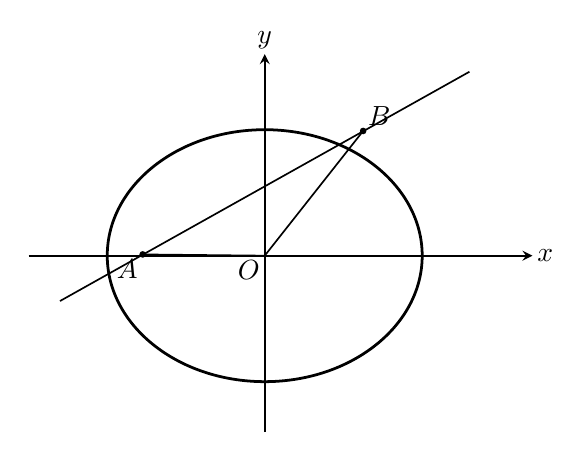
\begin{tikzpicture}[x=1.0cm, y=1.6cm, semithick,
  every node/.style={inner sep=1.5pt}]

  \draw[->,>=stealth] (-3.0,0) -- (3.4,0) node[right] {$x$};
  \draw[->,>=stealth] (0,-1.4) -- (0,1.6) node[above] {$y$};
  \node[below left] at (0,0) {$O$};

  % 椭圆 x^2/4+y^2=1
  \draw[line width=1pt] (0,0) ellipse (2 and 1);

  % 割线 y = 0.35x + 0.55（示意）
  \draw (-2.6,-0.36) -- (2.6,1.46);
  \coordinate (A) at (-1.55,0.01);
  \coordinate (B) at (1.25,0.99);
  \fill (A) circle (1.2pt);
  \fill (B) circle (1.2pt);
  \node[below left] at (A) {$A$};
  \node[above right] at (B) {$B$};

  \draw (A) -- (0,0) -- (B);
\end{tikzpicture}
\end{center}
\nopagebreak[4]
\Needspace{4\baselineskip}
\textbf{解析}

\Needspace{5\baselineskip}
（1）$k=0$ 时直线 $y=b$，与椭圆交于

\nopagebreak[4]
\[x=\pm2\sqrt{1-b^2}.\]

\Needspace{5\baselineskip}
三角形底 $AB=4\sqrt{1-b^2}$，高 $b$，故

\nopagebreak[4]
\[S=\frac12\cdot4\sqrt{1-b^2}\cdot b=2b\sqrt{1-b^2}.\]

\Needspace{5\baselineskip}
由 $b^2(1-b^2)\leqslant\dfrac14$，得

\nopagebreak[4]
\[S\leqslant2\cdot\frac12=1,\]

等号当 $b^2=\dfrac12$ 时成立。最大值 $1$。

\Needspace{5\baselineskip}
（2）设交点横坐标 $x_1$，$x_2$。由

\nopagebreak[4]
\[x^2/4+(kx+b)^2=1\]

\Needspace{5\baselineskip}
得

\nopagebreak[4]
\[\left(\frac14+k^2\right)x^2+2kbx+b^2-1=0.\]

\Needspace{5\baselineskip}
记 $D=k^2+\dfrac14$，则

\nopagebreak[4]
\[|x_1-x_2|=\frac{\sqrt{4k^2+1-b^2}}{D}.\]

\Needspace{5\baselineskip}
于是

\nopagebreak[4]
\[|AB|=\sqrt{1+k^2}|x_1-x_2|=2,\]

\nopagebreak[4]
\[S=\frac12|b||x_1-x_2|=1.\]

\Needspace{5\baselineskip}
两式相除得

\nopagebreak[4]
\[\frac{\sqrt{1+k^2}}{|b|}=1\ \Rightarrow\ b^2=1+k^2.\]

\Needspace{5\baselineskip}
代回 $|AB|$ 式：

\nopagebreak[4]
\[\sqrt{1+k^2}\cdot\frac{\sqrt{3k^2}}{k^2+\frac14}=2.\]

\Needspace{5\baselineskip}
化简得

\nopagebreak[4]
\[(k^2-\tfrac12)^2=0\ \Rightarrow\ k^2=\frac12,\qquad b^2=\frac32.\]

\Needspace{5\baselineskip}
故

\nopagebreak[4]
\[k=\pm\frac{\sqrt2}{2},\qquad b=\pm\frac{\sqrt6}{2},\]

\Needspace{5\baselineskip}
直线方程为

\nopagebreak[4]
\[y=\pm\frac{\sqrt2}{2}x\pm\frac{\sqrt6}{2}.\]

\gkanswer{答案：（1）$1$；（2）$y=\pm\dfrac{\sqrt2}{2}x\pm\dfrac{\sqrt6}{2}$。}

\end{answer}